% !Mode:: "TeX:UTF-8"
\chapter{SQLite数据库}

\section{SQLite简介}

SQLite,是一款轻型的数据库\upcite{junyan2009application},
是遵守ACID的关系型数据库管理系统,它包含在一个相对小的C库中。
它是D.RichardHipp建立的公有领域项目。
它的设计目标是嵌入式的,而且目前已经在很多嵌入式产品中使用了它,
它占用资源非常的低,在嵌入式设备中,可能只需要几百K的内存就够了。
它能够支持Windows/Linux/Unix等等主流的操作系统,同时能够跟很多程序语言相结合,
比如 Tcl、C\#、PHP、Java等,还有ODBC接口,
同样比起Mysql、PostgreSQL这两款开源的世界著名数据库管理系统来讲,它的处理速度比他们都快。
SQLite第一个Alpha版本诞生于2000年5月。 
至2016年已经有16个年头,SQLite重大更新的SQLite 3则更新于2015年。

不像常见的客户-服务器范例,SQLite引擎不是个程序与之通信的独立进程,
而是连接到程序中成为它的一个主要部分。所以主要的通信协议是在编程语言内的直接API调用。
这在消耗总量、延迟时间和整体简单性上有积极的作用。
整个数据库(定义、表、索引和数据本身)都在宿主主机上存储在一个单一的文件中。
它的简单的设计是通过在开始一个事务的时候锁定整个数据文件而完成的。

SQLite单文件的特性,使html5 filesystem API\upcite{bidelman2011using}
模拟实现有了理论上的可能。

\section{SQLite的程序的特征}

和lua虚拟机相同,SQLite我们也是需要得到一个“黑箱程序”即可。
但SQLite又和luaVM有个显著的不同,数据库都是C/S架构的,
我们需要在前端模拟实现C/S架构。

Html5中新增了原生的前端多线程方案,Web Worker\upcite{jarvinen2011html5},
依靠线程间通信,可以模拟实现C/S架构。

\section{SQLite的程序的移植过程}

\subsection{SQLite的程序的移植过程}

\begin{enumerate}
    \item 下载SQLite生成用c源码,只有一个c文件和一个头文件。
    \item 把sqlite3.c和sqlite3.h两个文件放在c文件夹下,然后编写如下makefile
\begin{verbatim}
# Need $(EMSCRIPTEN), for example run with        emmake make

EMSCRIPTEN?=/usr/bin

EMCC=$(EMSCRIPTEN)/emcc

CFLAGS=-DSQLITE_OMIT_LOAD_EXTENSION -DSQLITE_DISABLE_LFS -DLONGDOUBLE_TYPE=double -DSQLITE_INT64_TYPE="long long int" -DSQLITE_THREADSAFE=0

all: js/sql.js

debug: EMFLAGS= -O1 -g -s INLINING_LIMIT=10 
debug: js/sql-debug.js

optimized: EMFLAGS= --memory-init-file 0 --closure 1 -O3 -s INLINING_LIMIT=50
optimized: js/sql-optimized.js

js/sql.js: optimized
	cp js/sql-optimized.js js/sql.js

js/sql%.js: js/shell-pre.js js/sql%-raw.js js/shell-post.js
	cat $^ > $@

js/sql%-raw.js: c/sqlite3.bc js/api.js exported_functions
	$(EMCC) $(EMFLAGS) -s EXPORTED_FUNCTIONS=@exported_functions c/sqlite3.bc --post-js js/api.js -o $@

js/api.js: coffee/api.coffee coffee/exports.coffee coffee/api-data.coffee
	coffee --bare --compile --join $@ --compile $^

# Web worker API
worker: js/worker.sql.js
js/worker.js: coffee/worker.coffee
	coffee --bare --compile --join $@ --compile $^

js/worker.sql.js: js/sql.js js/worker.js
	cat $^ > $@

c/sqlite3.bc: c/sqlite3.c
	# Generate llvm bitcode
	$(EMCC) $(CFLAGS) c/sqlite3.c -o c/sqlite3.bc

module.tar.gz: test package.json AUTHORS README.md js/sql.js
	tar --create --gzip $^ > $@

clean:
	rm -rf js/sql*.js js/api.js js/sql*-raw.js c/sqlite3.bc
\end{verbatim}    	
	\item 运行make命令,得到sql.js文件
	\item 使用sql.js
\end{enumerate}



\subsection{SQLite的程序的移植过程分析}

\begin{enumerate}
    \item 把sqlite.c文件编译成sqlite.bc文件,即为llvm的字节码
    \item api.coffee,exports.coffee,api-data.coffee文件编译成api.js,coffeescript是一种脚本语言,可以编译成JavaScript,写作方式类似python
    \item sqlite.bc编译成sql-optimized-raw.js,需要api.js辅助
	\item 把shell-pre.js,sql-optimized-raw.js,shell-post.js合并,其中shell-pre和shell-post两个js文件是用来修饰SQLite的使用方法,使之在html和node.js中调用更方便
	\item 优化sql-optimized-raw.js,得到sql-optimized.js
	\item 将sql-optimized.js改名为sql.js
\end{enumerate}

\subsection{SQLite在浏览器中的运行效果}

图\ref{sqlite-html}展示了SQLite在浏览器中运行的效果。

\begin{figure}[h!] % [h!] 表示尽量排在当前位置
    \centering
    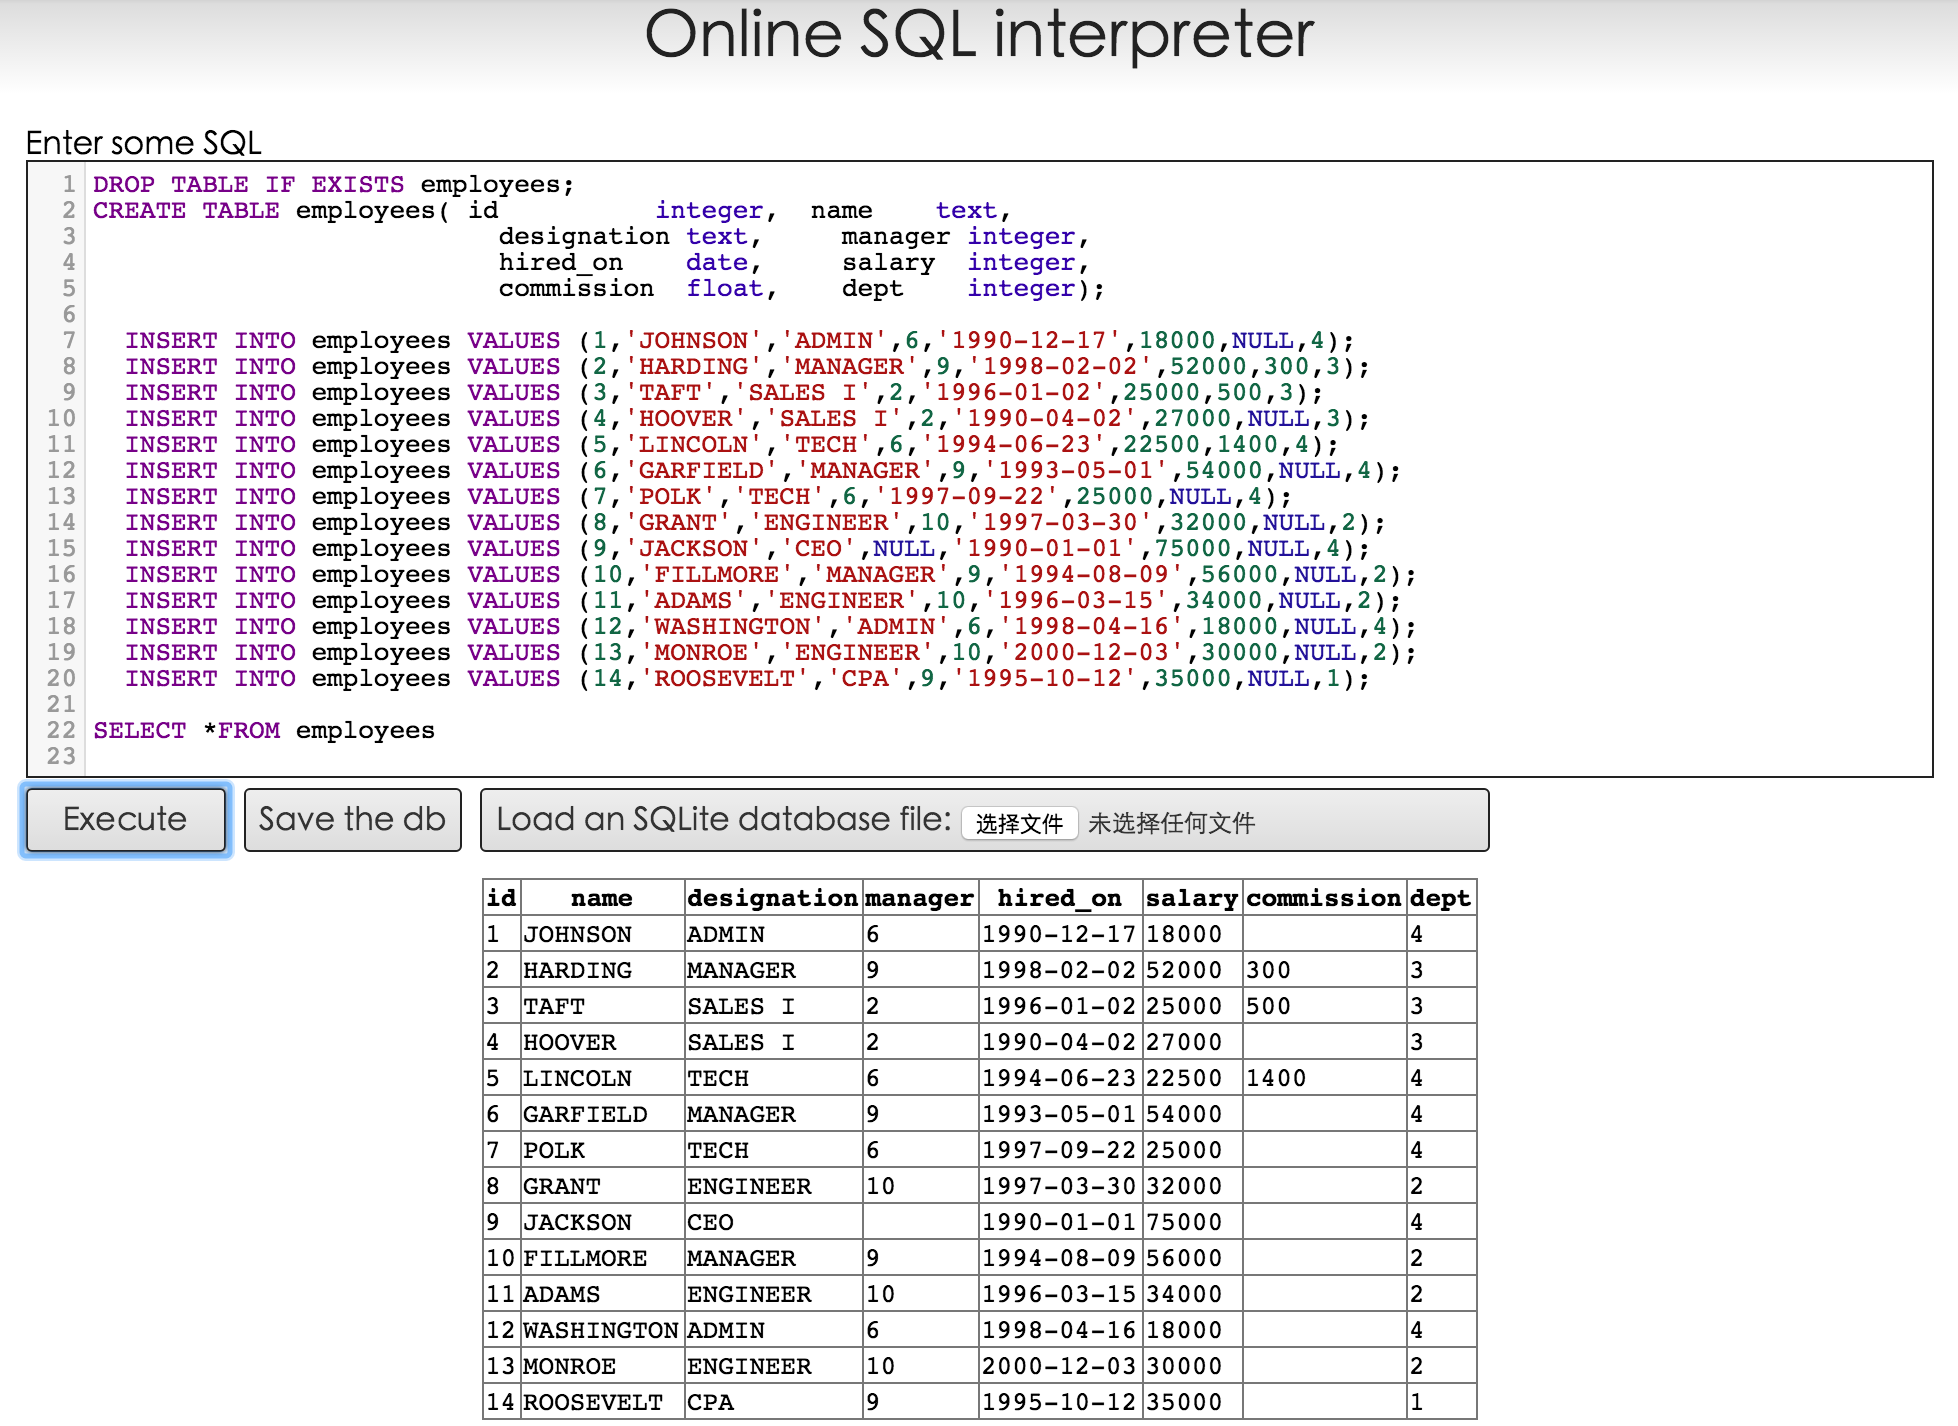
\includegraphics[width=450bp]{figure/pic/sqlite-sample-html.png}
    \caption{SQLite在浏览器中运行效果}
    \label{sqlite-html}
\end{figure}